\section{Experimental Evaluation}
\label{sec:eval}

%Opening is deliberately short because we gonna be running out of space 
In this section, we present empirical and analytical evaluation of the performance and cost of \sysname under different workloads and scales. 
Our evaluation consists of empirical analysis of the different scientific computing applications, as well as model-driven simulations for analyzing and comparing \sysname behavior under different preemption and application dynamics. 

% \begin{itemize}
% \item What is performance and cost of 
% \end{itemize}

\noindent \textbf{Environment and Workloads:} All our empirical evaluation is conducted on the Google Public Cloud, and with these representative scientific applications: 
% open-source
\vspace*{\tightext}
\begin{description}
  %TODO: Need MAX two sentence descriptions
\item[NC.] The ions in nanoconfiment~\cite{} application computes dynamics of nanoparticles. Uses OpenMP and MPI parallelization. 
\item[Shapes.]  Application to compute shapes of nanoparticles. Uses OpenMP and MPI parallelization and is embarrassingly parallel. 
\item[Lulesh.] Popular hydrodynamics application with the default parameters. 
\end{description}
\vspace*{\tightext}
All applications use OpenMPI, are deployed on Slurm vXXX and 64-bit Ubuntu 18.04, and run on Google Cloud VMs with x86-64 Intel Broadwell CPUs. 
%Networking? 


\subsection{SciSpot Performance and Cost}

\subsubsection{Impact of server exploration}

As described in Section~\ref{sec:design}, applications can be deployed on multiple types of VMs in the cloud, with each VM type having a different ``size''.
In our evaluation of parallel scientific applications that are CPU intensive, we are primarily interested in the number of CPUs in a VM.

When an application requests a total number of CPUs to run each of its jobs, \sysname first runs its exploration phase to find the ``right'' VM for the application.
\sysname searches for the VM that minimizes the total expected cost of running the application, and this depends on  several factors such as the parallel structure of the application, the preemption probability and the associated job recomputation time, and the price of the VM.


Thus, even if the \emph{total} amount of resources (i.e., number of CPUs) per job is held constant, the total running time of an application depends on the choice of the VM, and the associated number of VMs required to meet the allocation constraint (Section~\ref{subsec:cost-model}).
%
With preemptible instances, the total running time of a job is composed of two factors: the ``base'' running time of the job without any preemptions, and the expected recomputation time which depends on the probability of job failure (Equation~\ref{eq:t1}). 

\begin{figure}
  \centering
  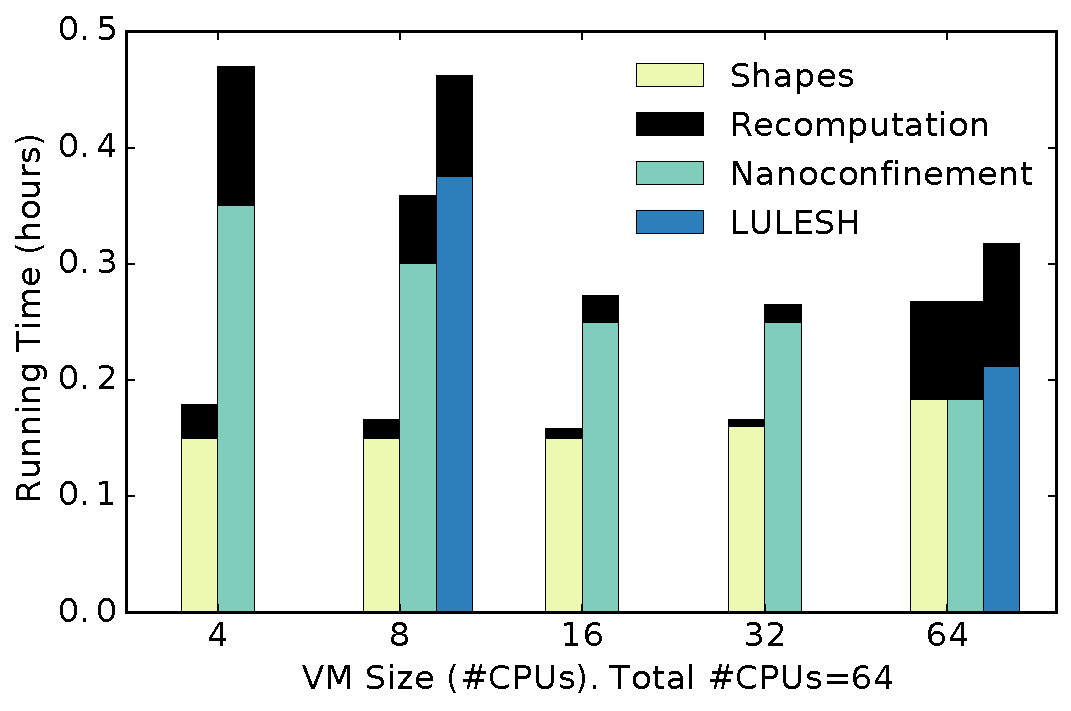
\includegraphics[width=0.4\textwidth]{../graphs/runtime-bars.pdf}
  \caption{Running times of applications on different VMs. The total number of CPUs is 64, yielding different number of VMs in each case. We see different tradeoffs in the base running times and recomputation costs for the different applications.}
  \label{fig:runtimes-bar}
\end{figure}


Figure~\ref{fig:runtimes-bar} shows the running times of the NC and Shapes application, when they are deployed on different VM sizes.
In all cases, the total number of CPUs per job is set to 64, and thus the different VM sizes yield different cluster sizes (e.g., 16 VMs with 4 CPUs each are required).


For the NC application, we observe that the the base running times (without preemptions) reduce when moving to larger VMs, because this entails lower communication costs.
The running time on the ``best'' VM (i.e., with 32 CPUs) is nearly 40\% lower as compared to the worst case. 
On the other hand, the Shapes application can scale to a larger number of VMs without any significant communication overheads, and does not see any significant change in its running time.

Figure~\ref{fig:runtimes-bar} also shows the total expected running time, that is obtained by adding the the expected recomputation time, which depends on the expected lifetimes of the VM and the number of VMs, and is computed using the cost model introduced in Section~\ref{subsec:cost-model}. 
While selecting larger VMs may reduce communication overheads and thus improve performance, it is not an adequate policy in the case of preemptible VMs, since the preemptions can significantly increase the total running time.
We can observe this in the case of NC application when deployed on a 64 CPU VM---even though the base running time is lower compared to deploying the application on 2x32-CPU VMs, the recomputation time on the 64 CPU VM is almost $4\times$ higher due to the much lower expected lifetime of the larger VMs. 
Thus, on preemptible servers, there is a tradeoff between the base running time which only considers parallelization overheads, and the recomputation time.
By considering \emph{both} these factors, \sysname's server selection policy can select the best VM for an application. 


\noindent \emph{\textbf{Result:} SciSpot's server selection, by considering both the base running time and recomputation time, can improve performance by up to 40\% , and can keep the increase in running time due to recomputation to less than 5\%.}


\subsubsection{Cost}

\begin{figure}
  \centering
  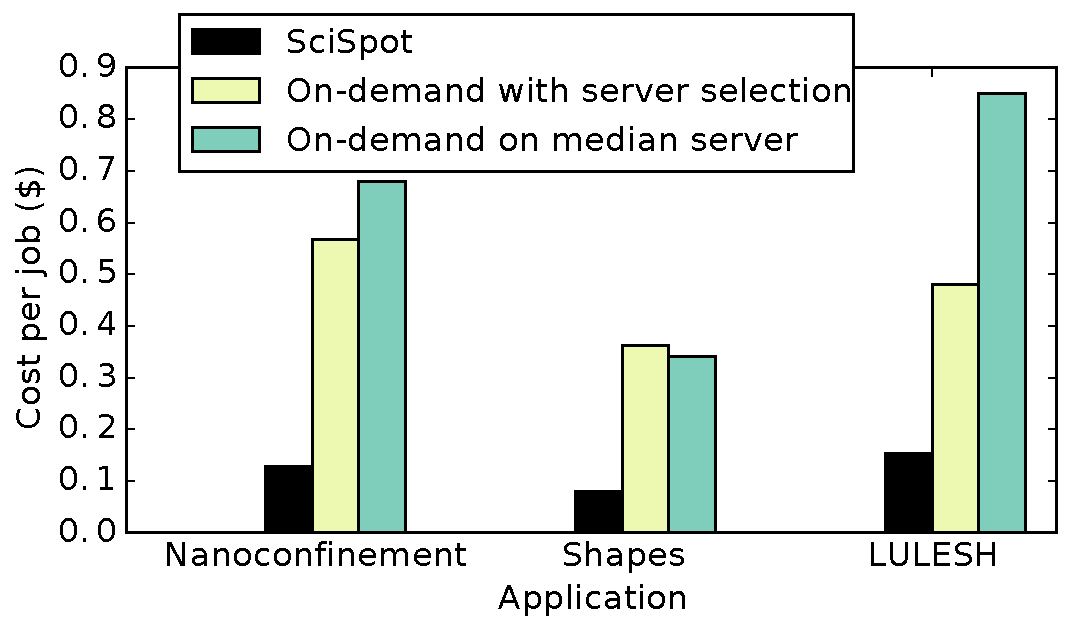
\includegraphics[width=0.4\textwidth]{../graphs/cost-only-bar.pdf}
  \caption{SciSpot's use of preemptible VMs can reduce costs by up to $5\times$ compared to conventional cloud deployments.}
  \label{fig:cost-only-bar}
\end{figure}


The primary motivation for using preemptible VMs is their significantly lower cost compared to conventional ``on-demand'' cloud VMs that are non-preemptible. 
Figure~\ref{fig:cost-only-bar} compares the cost of running different applications with different cloud VM deployments.
\sysname, which uses both cost-minimizing server selection, and preemptible VMs, results in significantly lower costs across the board, even when accounting for preemptions and recomputations. 
Even with \sysname's server selection, using on-demand VMs result in a $5\times$ cost increase.
In the absence of server selection, we assume that the user will pick a ``median'' VM in terms of number of CPUs (in this case, 8 CPU VMs), which we also show in Figure~\ref{fig:cost-only-bar}. 


\noindent \emph{\textbf{Result:} SciSpot reduces computing costs by up to 5x compared to conventional on-demand cloud deployments.}




\subsubsection{Comparison with HPC Clusters}

Scientific applications are typically run on large-scale HPC clusters, where different performance and cost dynamics apply.
While there are hardware differences between cloud VMs and HPC clusters that can contribute to performance differences, we are interested in the performance ``overheads''.
In the case of \sysname, the job failures and recomputations increase the total job running time, and are thus the main source of overhead.

On HPC clusters, jobs enjoy significantly lower recomputation probability, since the hardware on these clusters has MTTFs in the range of years to centuries~\cite{dongarra-ckpting}.
However, we emphasize that there exist \emph{other} sources of performance overheads in HPC clusters.
In particular, since HPC clusters have high resource utilization, they also have significant \emph{waiting} times. 
On the other hand, cloud resource utilization is low~\cite{borg} and there is usually no need to wait for resources, which is why transient servers exist in the first place! 


Thus, we compare the performance overhead due to preemptions for \sysname, and job waiting times in conventional HPC deployments.
To obtain the job waiting times in HPC clusters, we use the LANL Mustang traces published as part of the Atlas trace repository~\cite{cmu-atlas}.
We analyze the waiting time of over two million jobs submitted over a 5 year period, and compute the increase in running time of the job due to the job waiting or queuing time. 

\begin{figure}[t]
  \centering 
  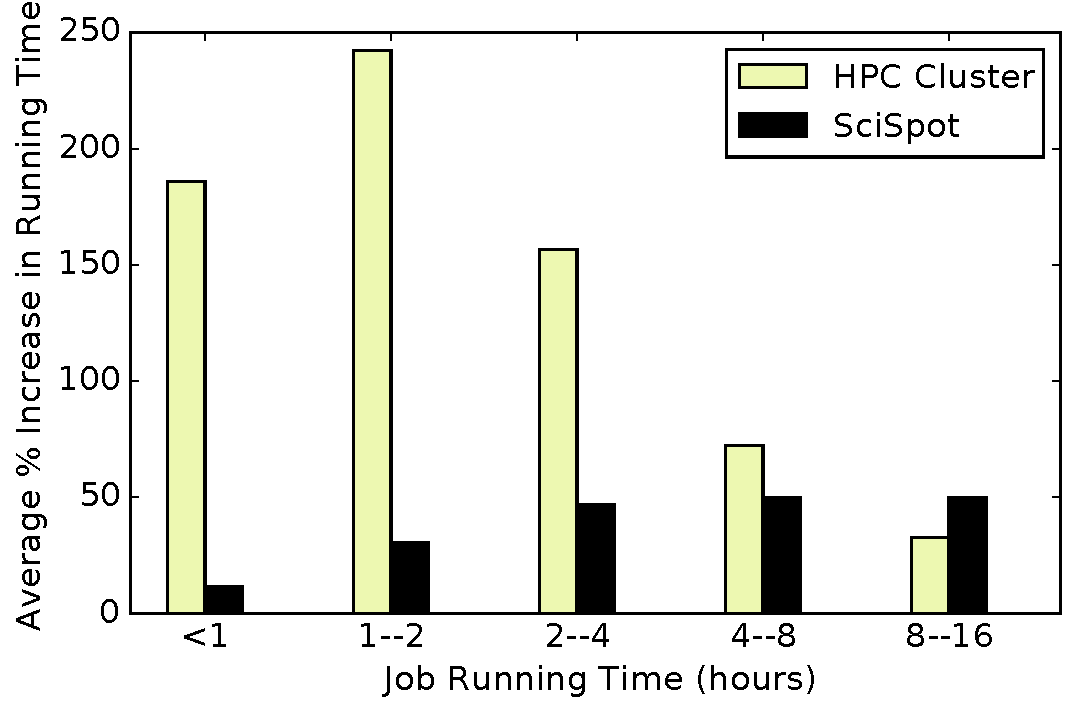
\includegraphics[width=0.4\textwidth]{../graphs/hpc-vs-scispot.pdf}
  \caption{Increase in running time due to waiting/queuing on HPC clusters is significantly higher than the recomputation time for \sysname, especially for shorter jobs. }
  \label{fig:hpc-vs-scispot}

\end{figure}


Figure~\ref{fig:hpc-vs-scispot} shows the increase in running time with \sysname, and due to waiting for resources in HPC clusters, for jobs of different lengths. We see that the average performance overhead due to waiting can be significant in the case of HPC clusters, and the job submission latency and queuing time dominate for smaller jobs, increasing their total running time by more $2.5\times$.
This waiting is amortized in the case of longer running jobs, and the increase in running time as a percentage drops off for longer jobs, to around 30\%.

On the other hand, \sysname's performance overhead is significantly smaller for jobs of up to 8 hours in length.
For longer jobs, the limited lifetime of Google Preemptible VMs (24 hours) begins to significantly increase the preemption probability and expected recomputation time.
We emphasize that these are \emph{individual} job lengths, and not the running time of entire bags of jobs.
We note that these large single jobs are rare, and for smaller jobs (within a much larger bag), both the preemption probability and recomputation overhead is much smaller.

\noindent \emph{ \textbf{Result:} While preemptions can increase running times due to recomputation, this increase is small, and is between 20 to 400\% lower compared to conventional HPC clusters. }


\subsection{SciSpot Scaling}


\begin{figure}
  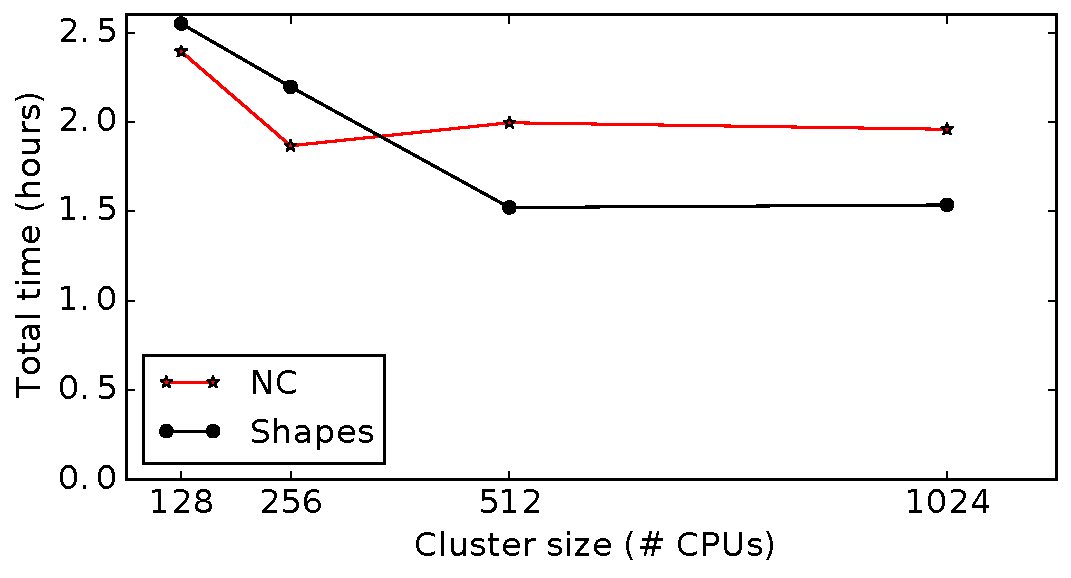
\includegraphics[width=0.4\textwidth]{../graphs/vm-per-job-scaling.pdf}
  \caption{SciSpot scaling as the VMs per jobs increases}
  \label{fig:vm-per-job-scaling}
\end{figure}

Figure~\ref{fig:vm-per-job-scaling} shows the total bag of job execution times for 32 jobs with 4 jobs running in parallel.
32 CPU VM's were used, and thus the total number of CPUs = 32*jobs-per-VM. Max CPU's used was 512 
Reach saturation because of the limitations of parallel speedup and coordination. 


\begin{figure}
  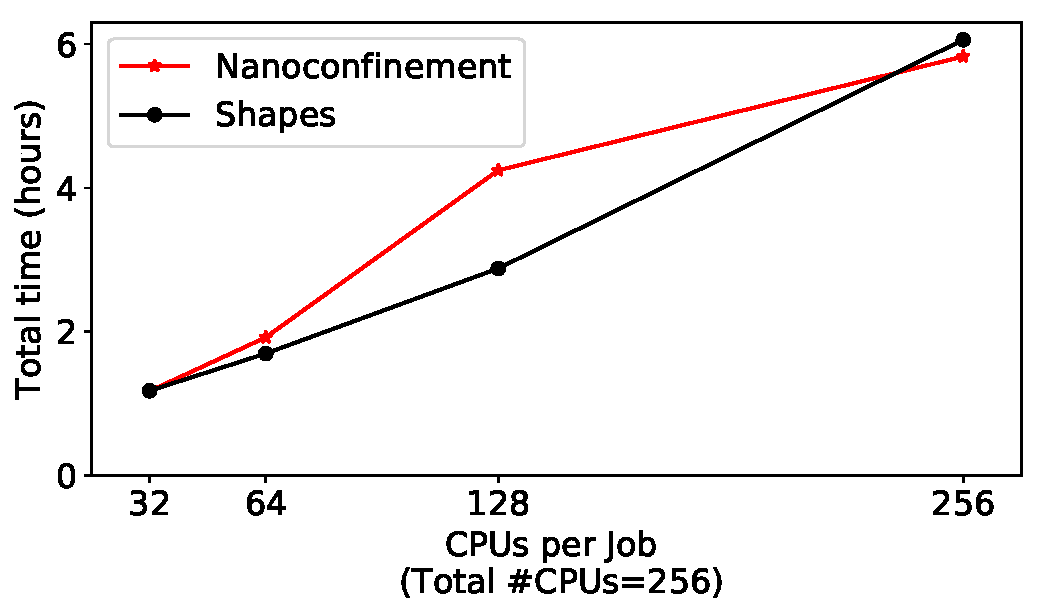
\includegraphics[width=0.3\textwidth]{../graphs/par-scaling.pdf}
  \caption{Job running times as the CPU's per job increases}
  \label{fig:par-scaling}
\end{figure}

Figure~\ref{fig:par-scaling} shows the running time when the total cluster size is fixed, but the number of parallel jobs and hence the number of CPUs per job changes. Smaller number of CPUs extracts higher parallel speedup and is thus recommended.


\noindent \textbf{Impact of Preemptions:} Figure~\ref{fig:fails-time} shows the total running time of the bag of jobs (32 jobs) for the nanoconfiment workload, when the total cluster size is 4 VMs. We ran the workload multiple times with different number of VM preemptions and hence jobs that failed. We see that even with a high number of preemptions, the running time only increases by about 30\%.
We note that this happens with a vanishingly small likelihood, for instance when the demand is very high and the preemptible VMs see high failure rates.
This shows that \sysname is robust and can provide acceptable performance even under extreme, adverse conditions. 

\begin{figure}[t]
  \centering 
  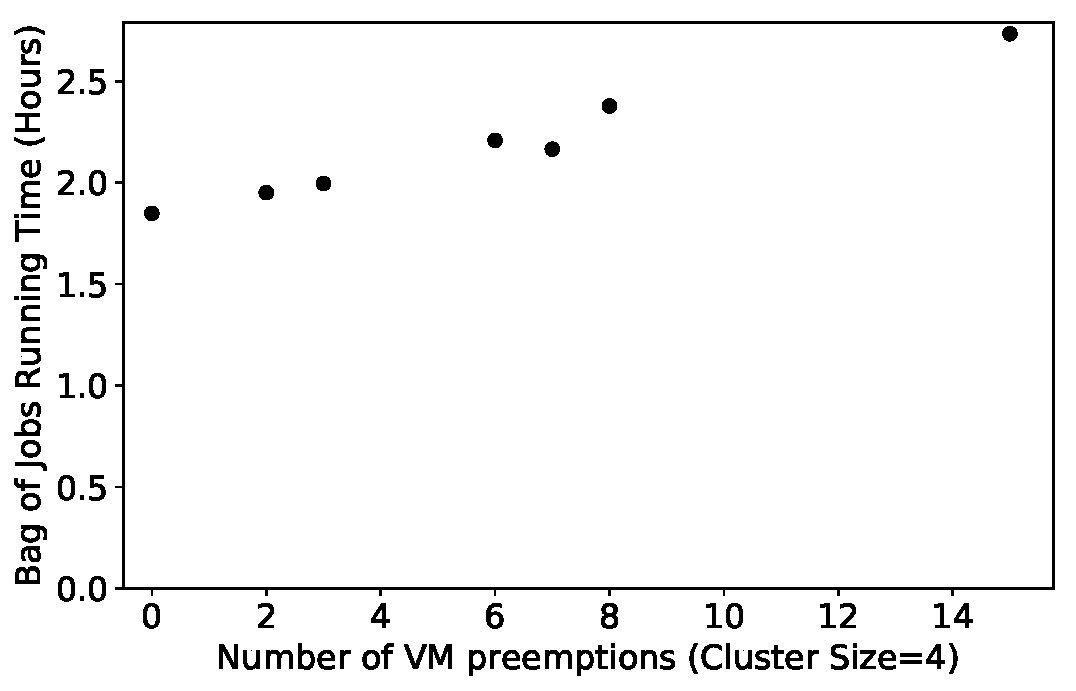
\includegraphics[width=0.4\textwidth]{../graphs/confin-fails-vs-time.pdf}
  \caption{The running time of a bag of 32 jobs increases by less than 40\%, even when the number of preemptions is high.}
  \label{fig:fails-time}
\end{figure}

\noindent \textbf{Large Bags:} Essentially time scalability. 4 Jobs in Parallel, each with 2 VMs each.  

%32_2_4 
\begin{table}
  \begin{tabular}{|c|r|r|}
    \hline
    Workload & Jobs & Time (Hours) \\
    \hline
    NC & 32  & 1.87 \\
    NC & 100  & 6.08 \\
    \hline
    Shapes & 32 & 1.47 \\
    Shapes & 100 & 4.49 \\  
    \hline
  \end{tabular}
  \caption{Running time for large, long-running bags of jobs.}
  \label{tab:100-jobs}
\end{table}



% \begin{figure}
%   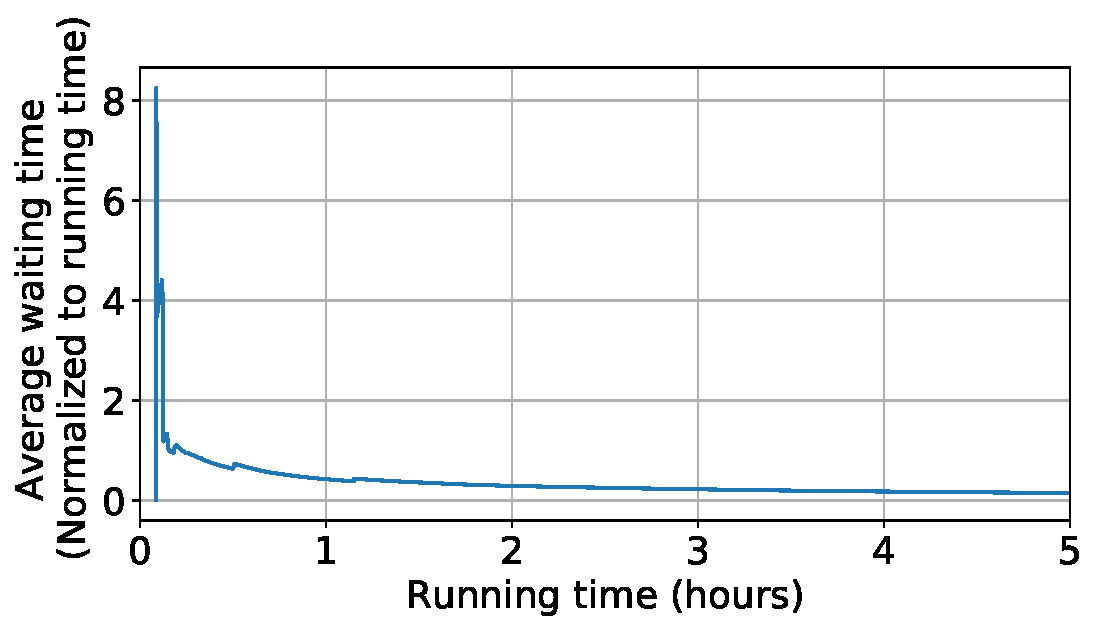
\includegraphics[width=0.4\textwidth]{../data/waiting_cumul.pdf}
%   \caption{The average waiting time (normalized to running time) of jobs of different length.}
%   \label{fig:hpc-wait-cdf}
% \end{figure}



%%% Local Variables:
%%% mode: latex
%%% TeX-master: "paper"
%%% End:
